\documentclass[12pt,a4paper]{report}

% Encodage et langue
\usepackage[utf8]{inputenc}
\usepackage[T1]{fontenc}
\usepackage[french]{babel}
\usepackage{lmodern}

% Mise en page
\usepackage{geometry}
\geometry{left=2.5cm,right=2.5cm,top=2.5cm,bottom=2.5cm}
\usepackage{setspace}
\onehalfspacing

% Figures, tableaux et liens
\usepackage{graphicx}
\usepackage{float}
\usepackage{array}
\usepackage{booktabs}
\usepackage{longtable}
\usepackage{tabularx}
\usepackage{xcolor}
\usepackage{caption}
\usepackage{xurl}
\usepackage{hyperref}
\usepackage{enumitem}
\usepackage{fancyhdr}
\usepackage{titlesec}
\usepackage{listings}

\graphicspath{{images/}}

\hypersetup{
    colorlinks=true,
    linkcolor=black,
    urlcolor=blue,
    citecolor=black,
    hypertexnames=false,
    pdftitle={Rapport PFA - AACA},
    pdfauthor={Azzdine El Hamdaoui}
}

\setcounter{tocdepth}{2}
\renewcommand{\contentsname}{Sommaire}
\renewcommand{\listfigurename}{Liste des figures}
\renewcommand{\listtablename}{Liste des tableaux}

\pagestyle{fancy}
\fancyhf{}
\lhead{\small AACA}
\rhead{\small Projet de Fin d'Année}
\cfoot{\thepage}
\setlength{\headheight}{14pt}

\titleformat{\chapter}[display]
  {\normalfont\bfseries\Huge}
  {\chaptername\ \thechapter}
  {20pt}
  {\Huge}

\lstset{
    basicstyle=\ttfamily\small,
    breaklines=true,
    frame=single,
    columns=fullflexible,
    backgroundcolor=\color{gray!5},
    keywordstyle=\color{blue!70!black},
    commentstyle=\color{green!40!black},
    stringstyle=\color{red!60!black}
}

% Informations du rapport
\newcommand{\university}{Université Sultan Moulay Slimane}
\newcommand{\school}{École Nationale des Sciences Appliquées -- Béni Mellal}
\newcommand{\field}{Cybersécurité et Intelligence Artificielle}
\newcommand{\level}{2\textsuperscript{ème} année du Cycle Ingénieur}
\newcommand{\projecttitle}{AACA : AI Academic Cognitive Assistant}
\newcommand{\projectsubtitle}{Assistant académique intelligent basé sur l'intelligence artificielle}
\newcommand{\studentname}{Azzdine El Hamdaoui}
\newcommand{\supervisor}{Ayoub Esswidi}
\newcommand{\academicyear}{2025--2026}

\begin{document}

% --------------------------------------------------------------------
% Page de garde
% --------------------------------------------------------------------
\begin{titlepage}
    \centering

    
\includegraphics[width=0.22\textwidth]{logo_ensabm.jpeg}\\[0.8cm]

    {\Large \textbf{\university}}\\[0.25cm]
    {\Large \textbf{\school}}\\[1.2cm]

    {\large Filière : \field}\\[0.25cm]
    {\large \level}\\[1.4cm]

    {\Huge \textbf{Rapport de Projet de Fin d'Année}}\\[1cm]

    {\LARGE \textbf{\projecttitle}}\\[0.35cm]
    {\large \projectsubtitle}\\[1.8cm]

    \begin{tabular}{rl}
        \textbf{Réalisé par :} & \studentname\\[0.35cm]
        \textbf{Encadré par :} & \supervisor\\
    \end{tabular}

    \vfill
    {\large Année universitaire : \academicyear}
\end{titlepage}

\pagenumbering{roman}
\setcounter{page}{1}

% --------------------------------------------------------------------
% Parties liminaires
% --------------------------------------------------------------------
\chapter*{Avant-propos}
\addcontentsline{toc}{chapter}{Avant-propos}

Dans le cadre de la formation d'ingénieur en \field{} à l'\school, le présent Projet de Fin d'Année a été réalisé afin de mettre en pratique les connaissances acquises en développement logiciel, intelligence artificielle, traitement de données et conception d'applications mobiles.

Le projet présenté dans ce rapport, intitulé \textbf{\projecttitle}, est une application mobile intelligente destinée aux étudiants. Il s'agit d'un projet académique personnel dont l'objectif est de transformer des captures de cours en ressources pédagogiques exploitables : texte structuré, résumé, quiz et flashcards.

Ce rapport présente le cheminement suivi depuis l'identification du besoin jusqu'à la réalisation technique de l'application. Il est organisé en trois chapitres afin de respecter les consignes du rapport : le premier chapitre expose le contexte et l'analyse des besoins, le deuxième décrit la conception et les choix technologiques, tandis que le troisième présente la réalisation, les tests et les résultats obtenus.

\chapter*{Dédicace}
\addcontentsline{toc}{chapter}{Dédicace}

Je dédie ce travail à ma famille, pour son soutien moral, sa patience et ses encouragements constants tout au long de mon parcours académique.

Je le dédie également à mes enseignants et à toutes les personnes qui ont contribué, directement ou indirectement, à ma formation et à l'aboutissement de ce projet.

\chapter*{Remerciements}
\addcontentsline{toc}{chapter}{Remerciements}

Je tiens à exprimer mes sincères remerciements à toutes les personnes qui ont contribué à la réalisation de ce travail.

Je remercie tout particulièrement mon encadrant, \textbf{\supervisor}, pour son accompagnement, ses orientations et ses remarques constructives tout au long de la préparation de ce projet.

Je remercie également l'ensemble du corps professoral et administratif de l'\school{} pour la qualité de la formation assurée, ainsi que mes collègues et proches pour leur soutien et leurs encouragements.

\chapter*{Résumé}
\addcontentsline{toc}{chapter}{Résumé}

Ce rapport présente la conception et la réalisation de \textbf{AACA} (\textit{AI Academic Cognitive Assistant}), une application mobile intelligente qui vise à aider les étudiants à mieux organiser, comprendre et réviser leurs cours. Le principe du projet est simple : l'étudiant capture une photo de ses notes ou d'un tableau, puis l'application extrait le contenu, le structure et génère automatiquement des supports pédagogiques tels qu'un résumé, des quiz et des flashcards.

Le système repose sur une architecture client-serveur. L'application mobile est développée avec \textbf{React Native} et \textbf{Expo}, tandis que le backend est construit avec \textbf{FastAPI}. Les données des utilisateurs, des notes, des quiz et des flashcards sont stockées dans \textbf{MongoDB}. Le traitement intelligent combine des modules d'OCR, de traitement d'image, de génération de contenu par modèles de langage, ainsi qu'un mécanisme de recherche sémantique basé sur des embeddings et une base vectorielle.

Le projet met également l'accent sur l'apprentissage actif grâce à la génération automatique de ressources de révision et à l'intégration d'un principe de répétition espacée pour les flashcards. La sécurité est prise en compte à travers une authentification par jetons JWT et une séparation claire entre les données des utilisateurs.

\textbf{Mots-clés :} intelligence artificielle, OCR, application mobile, apprentissage adaptatif, FastAPI, React Native, MongoDB, flashcards.

\tableofcontents
\listoffigures
\listoftables

\chapter*{Liste des abréviations}
\addcontentsline{toc}{chapter}{Liste des abréviations}

\begin{longtable}{p{3cm}p{11cm}}
\toprule
\textbf{Abréviation} & \textbf{Signification}\\
\midrule
AACA & AI Academic Cognitive Assistant\\
API & Application Programming Interface\\
CORS & Cross-Origin Resource Sharing\\
CRUD & Create, Read, Update, Delete\\
HTTP & HyperText Transfer Protocol\\
IA & Intelligence Artificielle\\
JSON & JavaScript Object Notation\\
JWT & JSON Web Token\\
LLM & Large Language Model\\
NLP & Natural Language Processing\\
OCR & Optical Character Recognition\\
PFA & Projet de Fin d'Année\\
RAG & Retrieval-Augmented Generation\\
REST & Representational State Transfer\\
SM-2 & SuperMemo Algorithm 2\\
UI/UX & User Interface / User Experience\\
\bottomrule
\end{longtable}

\clearpage
\pagenumbering{arabic}

% --------------------------------------------------------------------
% Introduction générale
% --------------------------------------------------------------------
\chapter*{Introduction générale}
\addcontentsline{toc}{chapter}{Introduction générale}

L'apprentissage universitaire repose encore largement sur des méthodes traditionnelles : prise de notes manuelle, capture de tableaux, relecture de documents et préparation individuelle de résumés. Ces pratiques restent utiles, mais elles deviennent rapidement difficiles à gérer lorsque le volume de cours augmente. Les étudiants accumulent souvent des photos, des fichiers et des notes dispersées, sans disposer d'un outil capable de transformer automatiquement ces contenus en supports de révision actifs.

En parallèle, les progrès récents de l'intelligence artificielle ont rendu possible l'analyse automatique d'images, l'extraction de texte, la compréhension de contenus académiques et la génération de ressources pédagogiques. Les modèles d'OCR permettent d'extraire du texte depuis des images, tandis que les grands modèles de langage peuvent reformuler, synthétiser et générer des questions à partir d'un contenu donné.

C'est dans ce contexte qu'a été conçu le projet \textbf{AACA}, pour \textit{AI Academic Cognitive Assistant}. L'idée principale est de proposer une application mobile capable de transformer une simple capture de cours en ressources pédagogiques structurées : résumé, contenu extrait, quiz et flashcards. Le projet vise ainsi à passer d'une prise de notes passive à une expérience d'apprentissage plus active, plus organisée et plus personnalisée.

Le présent rapport est structuré en trois chapitres. Le premier chapitre présente le contexte du projet, la problématique et l'analyse des besoins. Le deuxième chapitre décrit la conception du système, son architecture et les choix technologiques retenus. Le troisième chapitre expose la réalisation de l'application, le fonctionnement du backend et du frontend, ainsi que les tests et résultats obtenus.

% --------------------------------------------------------------------
% Chapitre 1
% --------------------------------------------------------------------
\chapter{Contexte général et analyse des besoins}

\section{Introduction}

Ce chapitre présente le cadre général du projet AACA. Il expose d'abord les difficultés rencontrées par les étudiants dans l'organisation et la révision de leurs cours, puis il formule la problématique principale du projet. Enfin, il identifie les besoins fonctionnels et non fonctionnels auxquels l'application doit répondre.

\section{Contexte du projet}

Dans l'environnement universitaire actuel, les étudiants manipulent une quantité importante d'informations : cours magistraux, travaux dirigés, supports PDF, notes personnelles, schémas, formules et photos de tableaux. Cette diversité rend l'organisation des connaissances de plus en plus complexe.

Une pratique fréquente consiste à prendre des photos du tableau ou du cahier afin de conserver rapidement une trace du cours. Cependant, ces captures restent souvent brutes : elles ne sont pas classées, ne sont pas recherchables et ne sont pas immédiatement exploitables pour la révision. L'étudiant doit ensuite relire, recopier, résumer et préparer lui-même des questions d'entraînement, ce qui demande du temps et une grande rigueur.

Par ailleurs, les méthodes d'apprentissage actif, telles que les quiz et les flashcards, sont reconnues pour favoriser la mémorisation. Pourtant, leur préparation reste manuelle et répétitive. Il existe donc un besoin réel d'un outil intelligent capable de relier directement la capture du cours à la génération de ressources de révision.

\section{Problématique}

La problématique centrale de ce projet peut être formulée comme suit :

\begin{quote}
Comment concevoir une application mobile intelligente capable de transformer automatiquement des captures de notes académiques en ressources d'apprentissage structurées, interactives et personnalisées ?
\end{quote}

Cette problématique soulève plusieurs défis : la qualité variable des images, la reconnaissance du texte, la compréhension du contenu extrait, la génération de ressources pédagogiques pertinentes et la protection des données personnelles de chaque utilisateur.

\section{Objectifs du projet}

L'objectif général du projet est de développer une application mobile intelligente permettant aux étudiants de capturer leurs notes de cours, d'en extraire automatiquement le contenu et de générer des ressources pédagogiques adaptées à la révision.

Les objectifs spécifiques sont les suivants :

\begin{itemize}[label=--]
    \item permettre la création et la connexion sécurisée des utilisateurs ;
    \item capturer ou importer une image contenant des notes de cours ;
    \item appliquer un prétraitement afin d'améliorer la lisibilité de l'image ;
    \item extraire automatiquement le texte à l'aide d'un système OCR ;
    \item corriger et structurer le texte extrait ;
    \item identifier la matière ou le domaine du contenu ;
    \item générer un résumé pédagogique ;
    \item générer des quiz interactifs ;
    \item générer des flashcards pour faciliter la révision ;
    \item sauvegarder les notes et ressources dans un espace personnel ;
    \item proposer un suivi de progression et des recommandations.
\end{itemize}

\section{Étude de l'existant}

Plusieurs outils permettent déjà de répondre partiellement au besoin. Google Lens permet d'extraire du texte à partir d'une image, mais ne propose pas une transformation pédagogique complète. Quizlet facilite la création et la révision de flashcards, mais la préparation du contenu reste souvent manuelle. Notion AI et ChatGPT peuvent aider à résumer ou expliquer un contenu, mais ils ne sont pas conçus comme une chaîne intégrée allant de la capture d'une image à la génération de supports de révision.

Ces solutions restent donc fragmentées. L'étudiant doit passer d'un outil à un autre : capturer l'image, extraire le texte, copier le contenu, demander un résumé, générer des questions, puis organiser les cartes de révision. Le projet AACA propose de centraliser ces étapes dans une seule application mobile, avec une expérience plus fluide.

\section{Analyse des besoins}

\subsection{Diagramme des cas d'utilisation}

Le diagramme des cas d'utilisation présente les principales interactions entre l'étudiant, l'application et le système d'intelligence artificielle. Il met en évidence les fonctions accessibles directement par l'utilisateur ainsi que les traitements déclenchés automatiquement par le système.

\begin{figure}[H]
    \centering
    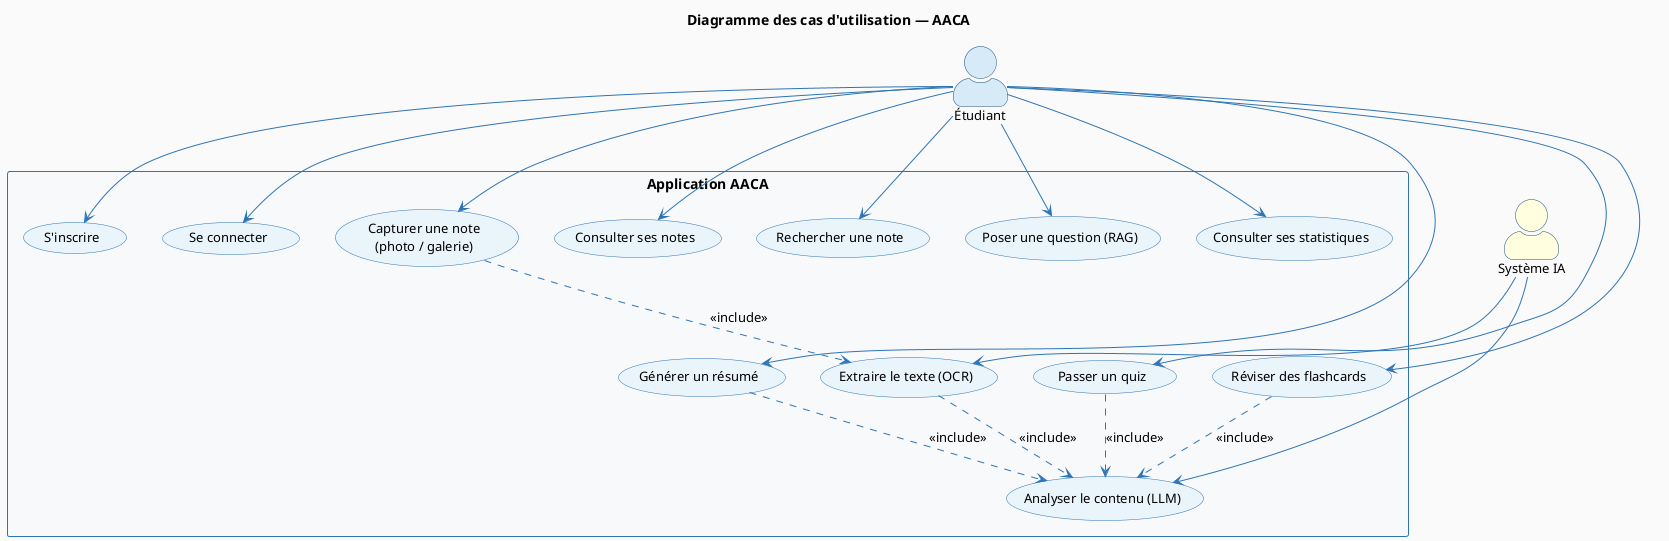
\includegraphics[width=\textwidth]{diagramme_cas_utilisation.png}
    \caption{Diagramme des cas d'utilisation de l'application AACA}
    \label{fig:cas-utilisation}
\end{figure}

\subsection{Besoins fonctionnels}

L'analyse des besoins permet d'identifier les modules fonctionnels suivants :

\begin{itemize}[label=--]
    \item \textbf{Gestion du compte :} inscription, connexion, authentification par jeton et gestion du profil utilisateur.
    \item \textbf{Capture et traitement :} capture d'une image depuis la caméra ou importation depuis la galerie, puis envoi vers le backend.
    \item \textbf{Extraction du contenu :} prétraitement de l'image, OCR, correction du texte et classification de la matière.
    \item \textbf{Génération pédagogique :} génération de résumés, quiz et flashcards à partir du contenu extrait.
    \item \textbf{Consultation des notes :} affichage de la liste des notes, consultation du détail, suppression ou modification.
    \item \textbf{Recherche :} recherche par mots-clés dans les notes enregistrées.
    \item \textbf{Révision :} passage de quiz et révision des flashcards.
    \item \textbf{Progression :} consultation de statistiques et recommandations personnalisées.
\end{itemize}

\subsection{Besoins non fonctionnels}

Au-delà des fonctionnalités visibles, l'application doit répondre à plusieurs exigences de qualité :

\begin{itemize}[label=--]
    \item \textbf{Sécurité :} protéger l'accès aux ressources personnelles à travers une authentification robuste.
    \item \textbf{Ergonomie :} proposer une interface simple, claire et adaptée à un usage mobile.
    \item \textbf{Performance :} réduire autant que possible le temps de traitement d'une image.
    \item \textbf{Extensibilité :} permettre l'ajout futur de nouveaux moteurs OCR, modèles IA ou fonctionnalités pédagogiques.
    \item \textbf{Maintenabilité :} organiser le code en modules séparés et compréhensibles.
    \item \textbf{Compatibilité :} viser un fonctionnement sur Android, iOS et éventuellement web via Expo.
\end{itemize}

\section{Conclusion}

Ce premier chapitre a présenté le besoin auquel répond AACA : transformer des notes académiques brutes en ressources pédagogiques utiles. La problématique met en évidence la nécessité d'un outil complet, combinant capture mobile, extraction de texte, intelligence artificielle et apprentissage actif. Ces besoins servent de base à la conception du système détaillée dans le chapitre suivant.

% --------------------------------------------------------------------
% Chapitre 2
% --------------------------------------------------------------------
\chapter{Conception et architecture du système}

\section{Introduction}

Ce chapitre décrit la conception générale de l'application AACA. Il présente l'architecture globale, les principaux composants du système, les diagrammes de conception et le modèle de données. L'objectif est de montrer comment les besoins identifiés précédemment ont été traduits en une architecture logicielle cohérente.

\section{Architecture globale}

\subsection{Principe général}

AACA repose sur une architecture client-serveur. L'application mobile représente la couche de présentation et permet à l'utilisateur d'interagir avec le système. Le backend FastAPI constitue la couche métier : il reçoit les requêtes, vérifie l'identité de l'utilisateur, orchestre le pipeline de traitement et communique avec les services d'intelligence artificielle. Enfin, la couche de persistance assure le stockage des utilisateurs, des notes, des quiz, des flashcards et des fichiers associés.

Cette séparation permet de maintenir une application mobile légère, tandis que les traitements coûteux, comme l'OCR ou la génération de contenu, sont centralisés côté serveur.

\subsection{Diagramme d'architecture}

\begin{figure}[H]
    \centering
    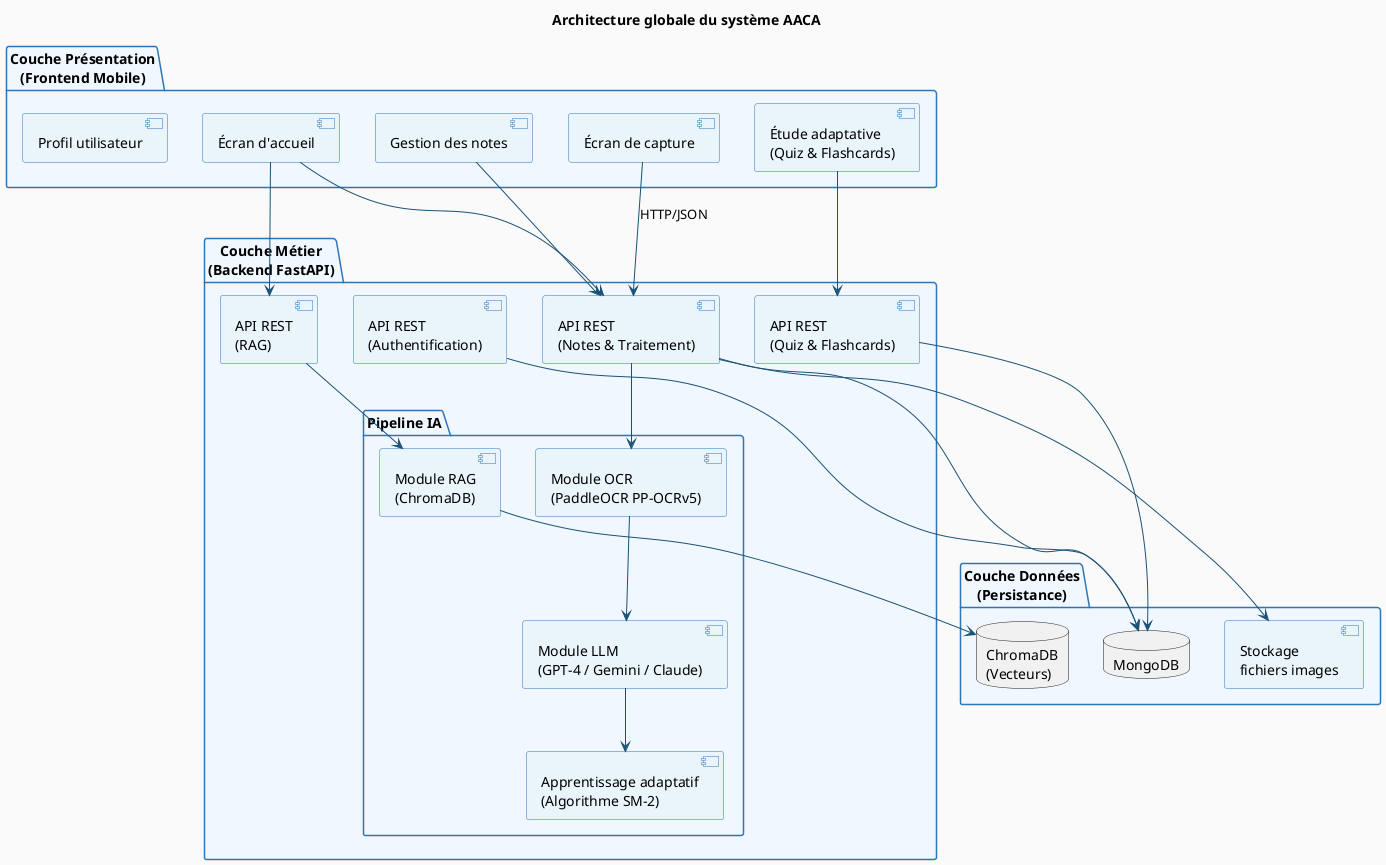
\includegraphics[width=\textwidth]{architecture_globale.png}
    \caption{Architecture globale du système AACA}
    \label{fig:architecture}
\end{figure}

\subsection{Couches de l'application}

L'architecture peut être divisée en trois grandes couches :

\begin{itemize}[label=--]
    \item \textbf{Couche présentation :} application mobile React Native/Expo, écrans d'authentification, accueil, capture, notes, étude et profil.
    \item \textbf{Couche métier :} API FastAPI, services de sécurité, pipeline OCR/IA, génération de ressources pédagogiques, apprentissage adaptatif.
    \item \textbf{Couche données :} MongoDB pour les données structurées, stockage local pour les fichiers et ChromaDB pour la recherche sémantique.
\end{itemize}

\section{Modélisation UML}

\subsection{Diagramme de classes}

Le diagramme de classes présente les principales entités manipulées par le système. L'utilisateur possède plusieurs notes. Chaque note peut être associée à des quiz et des flashcards. Les résultats des quiz permettent d'évaluer la progression de l'étudiant.

\begin{figure}[H]
    \centering
    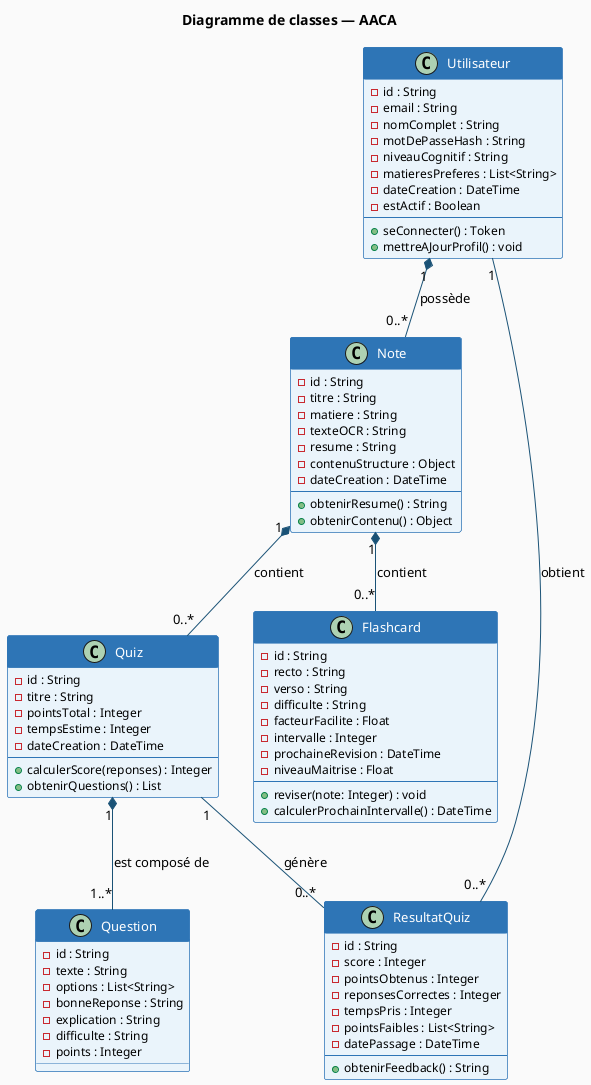
\includegraphics[height=0.82\textheight]{diagramme_classes.png}
    \caption{Diagramme de classes de l'application AACA}
    \label{fig:classes}
\end{figure}

\subsection{Diagramme de séquence}

Le diagramme de séquence décrit le scénario principal de capture et de traitement d'une note. L'étudiant prend une photo, l'application l'envoie au backend, le pipeline IA traite le contenu puis les résultats sont sauvegardés et retournés au frontend.

\begin{figure}[H]
    \centering
    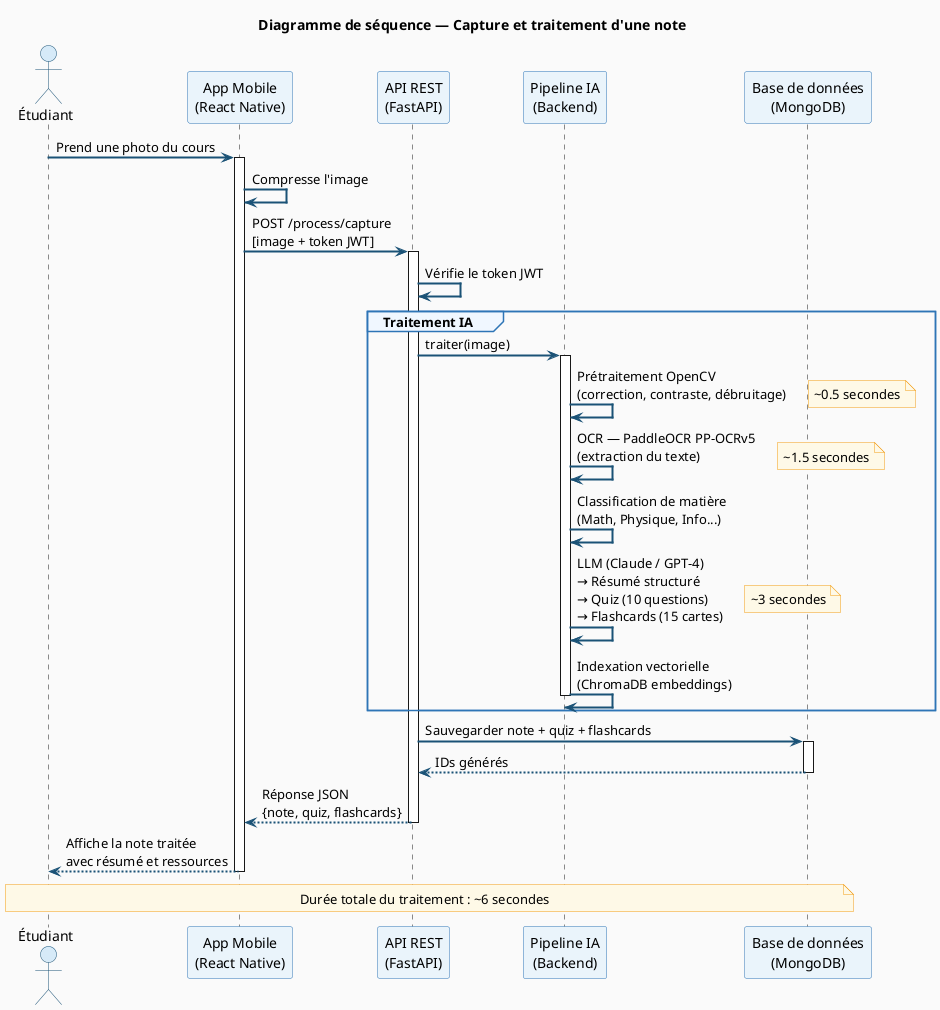
\includegraphics[height=0.82\textheight]{diagramme_sequence_capture.png}
    \caption{Diagramme de séquence : capture et traitement d'une note}
    \label{fig:sequence}
\end{figure}

\section{Modèle de données}

\subsection{Choix de MongoDB}

Le projet utilise MongoDB comme base de données principale. Ce choix est adapté à la nature des données manipulées : notes structurées, contenus extraits, quiz générés, flashcards, métadonnées de traitement et statistiques de progression. Ces données peuvent évoluer au cours du projet, ce qui rend une base NoSQL flexible particulièrement intéressante.

\subsection{Collections principales}

Les principales collections prévues sont les suivantes :

\begin{itemize}[label=--]
    \item \textbf{users :} informations des utilisateurs, mot de passe haché, niveau cognitif et préférences ;
    \item \textbf{notes :} titre, matière, texte brut, contenu structuré, résumé, formules et métadonnées ;
    \item \textbf{quizzes :} questions générées, réponses correctes, explications et difficulté ;
    \item \textbf{flashcards :} recto, verso, difficulté, date de prochaine révision et niveau de maîtrise ;
    \item \textbf{quiz\_results :} scores, réponses soumises, temps passé et recommandations ;
    \item \textbf{progress :} statistiques globales de l'utilisateur et historique d'activité.
\end{itemize}

\subsection{Recherche sémantique}

En complément de MongoDB, le projet prévoit une recherche sémantique basée sur les embeddings. Le contenu des notes peut être découpé en fragments, transformé en vecteurs numériques puis indexé dans une base vectorielle telle que ChromaDB. Cette approche facilite la recherche de passages proches du sens d'une question, et constitue une base pour des fonctionnalités de type RAG.

\section{Choix technologiques}

\begin{table}[H]
\centering
\begin{tabularx}{\textwidth}{|p{4cm}|p{3.5cm}|X|}
\hline
\textbf{Technologie} & \textbf{Catégorie} & \textbf{Rôle dans le projet}\\
\hline
React Native & Frontend mobile & Développement d'une application mobile multi-plateforme.\\
\hline
Expo & Outillage mobile & Gestion des permissions, de la caméra, du lancement et du développement mobile.\\
\hline
FastAPI & Backend Python & Création d'une API REST rapide, modulaire et documentée.\\
\hline
MongoDB & Base de données & Stockage des utilisateurs, notes, quiz, flashcards et résultats.\\
\hline
OpenCV & Traitement d'image & Amélioration de l'image, correction de perspective et prétraitement.\\
\hline
PaddleOCR / EasyOCR / Tesseract / OpenAI Vision & OCR & Extraction automatique du texte depuis les images.\\
\hline
LLM & IA générative & Génération de résumés, quiz, flashcards et corrections textuelles.\\
\hline
ChromaDB & Base vectorielle & Indexation sémantique des notes pour la recherche intelligente.\\
\hline
JWT & Sécurité & Authentification stateless entre le frontend et le backend.\\
\hline
\end{tabularx}
\caption{Technologies et outils utilisés dans le projet}
\label{tab:technologies}
\end{table}

\section{Pipeline de traitement}

Le pipeline de traitement constitue le coeur du backend. Il transforme une image brute en contenu pédagogique structuré à travers plusieurs étapes :

\begin{enumerate}
    \item réception de l'image envoyée par l'application mobile ;
    \item vérification du type et de la taille du fichier ;
    \item prétraitement de l'image : contraste, débruitage et correction éventuelle ;
    \item extraction du texte par OCR ;
    \item correction et structuration du texte extrait ;
    \item classification automatique de la matière ;
    \item génération du résumé, du quiz et des flashcards ;
    \item sauvegarde de la note et des ressources dans MongoDB ;
    \item indexation sémantique éventuelle dans la base vectorielle.
\end{enumerate}

Cette organisation modulaire facilite l'évolution du projet : il est possible de remplacer un moteur OCR, d'ajouter un nouveau fournisseur LLM ou d'améliorer le système de recommandations sans réécrire toute l'application.

\section{Sécurité}

La sécurité repose principalement sur l'authentification par jetons JWT. Lors de la connexion, le serveur génère un jeton d'accès et un jeton de rafraîchissement. Les routes protégées exigent un jeton valide afin d'empêcher l'accès non autorisé aux notes ou aux ressources d'un autre utilisateur.

Les mots de passe ne sont pas stockés en clair. Ils sont hachés avant l'enregistrement en base de données. De plus, le backend applique une vérification de propriété sur les ressources sensibles : une note, un quiz ou une flashcard ne peut être consulté ou modifié que par son propriétaire.

\section{Conclusion}

Ce chapitre a présenté la conception technique d'AACA. L'architecture client-serveur, le découpage en modules, le modèle de données et le pipeline de traitement permettent de répondre aux besoins exprimés dans le premier chapitre. La solution repose sur des technologies modernes et extensibles, adaptées à un projet combinant mobile, backend et intelligence artificielle.

% --------------------------------------------------------------------
% Chapitre 3
% --------------------------------------------------------------------
\chapter{Réalisation, tests et résultats}

\section{Introduction}

Ce chapitre présente la mise en oeuvre concrète du projet. Il décrit l'organisation du backend, les principales fonctionnalités de l'application mobile, les routes API développées, ainsi que les tests et résultats obtenus durant la validation.

\section{Réalisation du backend}

\subsection{Organisation du serveur}

Le backend est développé avec FastAPI. Il est structuré autour de plusieurs dossiers : les routes API, les modèles de données, les services métier et le noyau de configuration. Cette organisation permet de séparer clairement les responsabilités.

Les routes reçoivent les requêtes HTTP envoyées par l'application mobile. Les services assurent les traitements principaux : OCR, génération de contenu, stockage, recherche, apprentissage adaptatif et sécurité. Les modèles Pydantic définissent la forme des données échangées entre le backend et le frontend.

\subsection{Fonctionnalités de l'API}

\begin{table}[H]
\centering
\begin{tabularx}{\textwidth}{|p{3cm}|p{5cm}|X|}
\hline
\textbf{Méthode} & \textbf{Route} & \textbf{Description}\\
\hline
POST & /auth/register & Créer un compte utilisateur.\\
\hline
POST & /auth/login & Se connecter et obtenir les jetons JWT.\\
\hline
POST & /auth/refresh & Générer un nouveau jeton d'accès.\\
\hline
POST & /process/image & Traiter une image sans l'enregistrer comme note.\\
\hline
POST & /process/capture & Capturer, traiter et sauvegarder une note.\\
\hline
GET & /notes & Récupérer les notes de l'utilisateur.\\
\hline
GET & /notes/\{id\} & Consulter le détail d'une note.\\
\hline
PATCH & /notes/\{id\} & Modifier les métadonnées d'une note.\\
\hline
DELETE & /notes/\{id\} & Supprimer une note.\\
\hline
POST & /notes/\{id\}/summary & Générer un nouveau résumé.\\
\hline
POST & /notes/\{id\}/quizzes & Générer un quiz pour une note.\\
\hline
POST & /quizzes/\{id\}/submit & Soumettre les réponses d'un quiz.\\
\hline
GET & /notes/\{id\}/flashcards & Récupérer les flashcards d'une note.\\
\hline
POST & /flashcards/\{id\}/review & Réviser une flashcard et calculer la prochaine révision.\\
\hline
GET & /user/progress & Consulter la progression de l'utilisateur.\\
\hline
GET & /stats & Consulter des statistiques générales.\\
\hline
\end{tabularx}
\caption{Principales fonctionnalités de l'API AACA}
\label{tab:api}
\end{table}

\subsection{Pipeline IA}

Lorsqu'une image est envoyée à l'API, le pipeline commence par la validation du fichier. L'image est ensuite prétraitée afin d'améliorer sa qualité. Le service OCR extrait le texte, puis le service de correction améliore le contenu extrait. Le sujet est ensuite détecté automatiquement ou fixé à partir d'un indice fourni par l'utilisateur.

Lorsque les services d'intelligence artificielle sont disponibles, le backend génère un résumé, un quiz et des flashcards. Les résultats sont associés à l'utilisateur connecté et sauvegardés en base de données. Ce processus permet à l'étudiant de retrouver immédiatement la note traitée dans son espace personnel.

\subsection{Révision espacée}

Les flashcards sont utilisées pour favoriser la mémorisation à long terme. Après chaque révision, l'utilisateur indique le niveau de difficulté ressenti. Cette note permet au système de calculer la prochaine date de révision. Une carte difficile est reproposée rapidement, tandis qu'une carte maîtrisée peut être espacée dans le temps.

\section{Réalisation du frontend}

\subsection{Organisation générale}

L'application mobile est développée avec React Native et Expo. La navigation est gérée par Expo Router, qui permet d'organiser les écrans à partir de l'arborescence des fichiers. Les contextes React centralisent l'état global de l'application : authentification, notes et session d'étude.

\subsection{Écrans principaux}

L'application contient plusieurs écrans principaux :

\begin{itemize}[label=--]
    \item \textbf{Écran de connexion et inscription :} accès sécurisé à l'espace utilisateur.
    \item \textbf{Accueil :} aperçu des notes récentes et de l'activité de révision.
    \item \textbf{Capture :} prise de photo ou import d'image, puis envoi au backend.
    \item \textbf{Notes :} liste des notes sauvegardées avec recherche et filtres.
    \item \textbf{Détail d'une note :} consultation du résumé, du contenu extrait et des outils d'étude.
    \item \textbf{Étude :} affichage des quiz et des flashcards.
    \item \textbf{Profil :} informations utilisateur, préférences et changement de mot de passe.
\end{itemize}

\subsection{Gestion de l'authentification}

Après la connexion, le frontend conserve le jeton d'accès et le jeton de rafraîchissement. À chaque requête protégée, le jeton d'accès est envoyé dans l'en-tête HTTP. En cas d'expiration, l'application tente d'obtenir un nouveau jeton à partir du jeton de rafraîchissement. Cette approche améliore l'expérience utilisateur tout en conservant un niveau de sécurité satisfaisant.

\subsection{Expérience utilisateur}

L'interface mobile a été pensée pour guider rapidement l'étudiant vers les actions essentielles : capturer une note, consulter ses cours et réviser. L'utilisation d'icônes, de cartes, de filtres et d'indicateurs de progression rend l'expérience plus claire. Le projet intègre également une gestion de thème afin d'adapter l'affichage aux préférences de l'utilisateur.

\section{Tests et validation}

\subsection{Approche de validation}

La validation du projet repose sur deux niveaux : des tests fonctionnels manuels pour vérifier les scénarios principaux de l'application, et des tests automatisés côté backend pour contrôler les services critiques tels que l'authentification, les notes, les quiz, les flashcards et la sécurité d'accès.

Les tests ont notamment porté sur les cas suivants :

\begin{itemize}[label=--]
    \item création d'un compte utilisateur ;
    \item connexion avec des identifiants valides ;
    \item accès à une route protégée avec un jeton JWT ;
    \item capture et traitement d'une image ;
    \item création et consultation d'une note ;
    \item génération d'un quiz ;
    \item récupération et révision des flashcards ;
    \item recherche dans les notes ;
    \item protection contre l'accès aux données d'un autre utilisateur.
\end{itemize}

\subsection{Résultats de validation}

\begin{table}[H]
\centering
\begin{tabularx}{\textwidth}{|p{4.2cm}|X|p{2.5cm}|}
\hline
\textbf{Fonctionnalité} & \textbf{Résultat attendu} & \textbf{Statut}\\
\hline
Authentification & L'utilisateur peut créer un compte, se connecter et accéder aux routes protégées. & Validé\\
\hline
Capture image & L'utilisateur peut sélectionner ou prendre une photo et l'envoyer au backend. & Validé\\
\hline
Traitement OCR & Le texte est extrait à partir de l'image lorsque la qualité est suffisante. & Validé\\
\hline
Création de note & Une note est sauvegardée avec son titre, son contenu et ses métadonnées. & Validé\\
\hline
Résumé IA & Le système génère un résumé exploitable à partir du texte extrait. & Validé\\
\hline
Quiz & Le système génère des questions associées au contenu de la note. & Validé\\
\hline
Flashcards & Le système génère des cartes recto-verso pour la révision. & Validé\\
\hline
Recherche & L'utilisateur peut retrouver une note à partir d'un mot-clé. & Validé\\
\hline
Sécurité d'accès & Un utilisateur ne peut pas consulter ou modifier les ressources d'un autre utilisateur. & Validé\\
\hline
\end{tabularx}
\caption{Résultats des tests fonctionnels}
\label{tab:tests}
\end{table}

\subsection{Limites observées}

Même si le projet répond aux objectifs principaux, certaines limites doivent être mentionnées :

\begin{itemize}[label=--]
    \item la qualité de l'OCR dépend fortement de la netteté, de la luminosité et de l'angle de la photo ;
    \item la génération de résumé, quiz et flashcards dépend de la disponibilité des services IA configurés ;
    \item le traitement complet peut être plus long pour des images complexes ou volumineuses ;
    \item certaines statistiques de progression peuvent être enrichies dans une version future ;
    \item le mode hors ligne n'est pas encore complet, car plusieurs traitements nécessitent le backend et des services IA.
\end{itemize}

\section{Résultats obtenus}

Le résultat principal du projet est une application mobile fonctionnelle reliée à un backend FastAPI. L'utilisateur peut s'inscrire, se connecter, capturer une note, lancer le traitement intelligent et retrouver le contenu généré dans son espace personnel.

Le backend assure la gestion des utilisateurs, des notes, des quiz, des flashcards et de la progression. L'application mobile propose une interface claire pour consulter les notes et réviser les contenus générés. Le projet démontre ainsi l'intérêt de combiner OCR, IA générative et apprentissage actif dans un même système éducatif.

\section{Perspectives d'amélioration}

Plusieurs améliorations peuvent être envisagées :

\begin{itemize}[label=--]
    \item améliorer la précision OCR sur l'écriture manuscrite ;
    \item ajouter un mode hors ligne partiel pour consulter les notes déjà traitées ;
    \item permettre l'export des notes en PDF ou en Markdown ;
    \item ajouter un partage de notes entre étudiants ;
    \item enrichir le tableau de bord de progression avec des graphiques détaillés ;
    \item intégrer la transcription audio de cours enregistrés ;
    \item améliorer le système RAG pour permettre des questions/réponses plus avancées sur l'ensemble des notes.
\end{itemize}

\section{Conclusion}

Ce chapitre a présenté la réalisation concrète du projet AACA. Le backend, le frontend, le pipeline IA et les mécanismes de validation montrent que la solution proposée répond aux objectifs initiaux. Malgré certaines limites liées à la qualité des images et à la dépendance aux services IA, le projet constitue une base solide pour un assistant académique intelligent.

% --------------------------------------------------------------------
% Conclusion générale
% --------------------------------------------------------------------
\chapter*{Conclusion générale}
\addcontentsline{toc}{chapter}{Conclusion générale}

Le projet \textbf{AACA} montre comment l'intelligence artificielle peut être utilisée pour améliorer l'apprentissage des étudiants. En combinant une application mobile, un backend API, des moteurs OCR, des modèles de langage et une base de données, le système permet de transformer une simple capture de cours en supports pédagogiques utiles.

Les objectifs principaux ont été atteints : capture ou import d'image, extraction de texte, structuration du contenu, génération de résumé, création de quiz, génération de flashcards, sauvegarde des notes et consultation depuis l'application mobile. Le projet a également permis de mettre en pratique des compétences variées : développement mobile, développement backend, sécurité, bases de données, traitement d'image et intégration de services d'intelligence artificielle.

Ce travail représente une étape importante vers un assistant académique plus complet. Les futures versions pourraient intégrer une meilleure prise en charge de l'écriture manuscrite, un mode hors ligne, l'export des contenus, une collaboration entre étudiants et des statistiques de progression plus avancées. AACA constitue ainsi une base prometteuse pour accompagner les étudiants dans une révision plus active, plus organisée et plus personnalisée.

% --------------------------------------------------------------------
% Bibliographie
% --------------------------------------------------------------------
\begin{thebibliography}{12}
\addcontentsline{toc}{chapter}{Bibliographie}

\bibitem{vaswani2017}
VASWANI, Ashish, et al. \textit{Attention is All You Need}. Advances in Neural Information Processing Systems, 2017.

\bibitem{lewis2020}
LEWIS, Patrick, et al. \textit{Retrieval-Augmented Generation for Knowledge-Intensive NLP Tasks}. NeurIPS, 2020.

\bibitem{ebbinghaus1885}
EBBINGHAUS, Hermann. \textit{Über das Gedächtnis}. Duncker \& Humblot, 1885.

\bibitem{wozniak1990}
WOZNIAK, Piotr. \textit{Optimization of Learning: A New Approach and Computer Application}. 1990.

\bibitem{fastapi}
FastAPI Documentation. \url{https://fastapi.tiangolo.com/}

\bibitem{reactnative}
React Native Documentation. \url{https://reactnative.dev/}

\bibitem{expo}
Expo Documentation. \url{https://docs.expo.dev/}

\bibitem{mongodb}
MongoDB Documentation. \url{https://www.mongodb.com/docs/}

\bibitem{paddleocr}
PaddleOCR Documentation. \url{https://github.com/PaddlePaddle/PaddleOCR}

\bibitem{chromadb}
ChromaDB Documentation. \url{https://docs.trychroma.com/}

\bibitem{openai}
OpenAI Documentation. \url{https://platform.openai.com/docs}

\bibitem{anthropic}
Anthropic Documentation. \url{https://docs.anthropic.com/}

\end{thebibliography}

% --------------------------------------------------------------------
% Annexes
% --------------------------------------------------------------------
\appendix
\chapter{Guide d'installation}

\section{Backend}

\begin{enumerate}
    \item Se placer dans le dossier du backend.
    \item Créer un environnement virtuel Python :
\begin{lstlisting}[language=bash]
python3 -m venv venv
source venv/bin/activate
\end{lstlisting}
    \item Installer les dépendances :
\begin{lstlisting}[language=bash]
pip install -r requirements.txt
\end{lstlisting}
    \item Copier le fichier de configuration :
\begin{lstlisting}[language=bash]
cp .env.example .env
\end{lstlisting}
    \item Renseigner les variables nécessaires : clé secrète, base de données MongoDB et clés API IA.
    \item Lancer MongoDB localement ou via Docker :
\begin{lstlisting}[language=bash]
docker run -d --name mongodb-aaca -p 27017:27017 mongo:7.0
\end{lstlisting}
    \item Démarrer le serveur :
\begin{lstlisting}[language=bash]
uvicorn app.main:app --reload
\end{lstlisting}
\end{enumerate}

\section{Frontend}

\begin{enumerate}
    \item Se placer dans le dossier frontend.
    \item Installer les dépendances :
\begin{lstlisting}[language=bash]
npm install
\end{lstlisting}
    \item Configurer l'adresse de l'API dans le fichier \texttt{.env} :
\begin{lstlisting}
EXPO_PUBLIC_API_URL=http://ADRESSE_IP:8000/api/v1
\end{lstlisting}
    \item Lancer l'application :
\begin{lstlisting}[language=bash]
npx expo start
\end{lstlisting}
    \item Scanner le QR code avec Expo Go ou lancer l'application sur un simulateur.
\end{enumerate}

\chapter{Extraits de code représentatifs}

\section{Structure simplifiée d'une route protégée}

\begin{lstlisting}[language=Python]
@router.get("/notes")
async def list_notes(current_user: str = Depends(get_current_user)):
    notes = await mongodb_service.get_user_notes(current_user)
    return notes
\end{lstlisting}

\section{Principe du pipeline de traitement}

\begin{lstlisting}[language=Python]
async def process_image(image_bytes, options):
    processed_image = await image_processor.preprocess(image_bytes)
    ocr_result = await ocr_service.extract_text(processed_image)
    corrected_text = ocr_service.correct_text(ocr_result["text"])
    summary = await llm_service.generate_summary(corrected_text)
    quiz = await llm_service.generate_quiz(corrected_text)
    flashcards = await llm_service.generate_flashcards(corrected_text)
    return summary, quiz, flashcards
\end{lstlisting}

\end{document}
